%\documentclass[reponses, utf8, 11pt]{feuille}
\documentclass[utf8, 11pt]{feuille}

\newcommand{\titredutd}{\textbf{TD7 --- L'ensemble canonique~: premières applications}}

\begin{document}


\begin{tcolorbox}[
        colback=gray!20,
        colframe=gray!20,
        width=\dimexpr\textwidth\relax, 
        arc=0pt,outer arc=0pt,
        ]

\texttt{Seules les calculatrices non communicantes et les notes manuscrites personnelles sont autorisées.}

\texttt{Les exercices sont totalement indépendants.}

\texttt{On notera $k_B$ la constante de Boltzmann et $h$ la constante de Planck.}

\end{tcolorbox}



% ______________________________________________________________________________
\section{\medium~Ortho et para hydrogène}

Dans son état électronique fondamental, la molécule d'hydrogène H$_2$ peut exister sous deux formes : l'ortho-hydrogène où les spins des deux noyaux sont parallèles et le para-hydrogène, où ils sont antiparallèles. La forme para possède un seul état de spin dont on prendra l'énergie comme origine; la forme ortho présente trois états distincts, de même énergie $\epsilon >0$. On considère un échantillon d'hydrogène solide, constitué de $N$ molécules, fixes et discernables, faiblement couplées. On ne s'intéresse qu'aux états de spin ortho et para. Ce cristal est en contact avec un thermostat à la
température $T$

%\elements{
%\\
%1 : $Z=z^N$ avec pour une molécule $z=\sum_{i=1}^4 {\rm e}^{-\beta \epsilon_i}=1+3{\rm e}^{-\beta \epsilon}$.
%\\
% 2 : $\langle E\rangle=-\frac{\partial \ln Z}{\partial \beta}=N \epsilon \frac{3{\rm e}^{-\beta \epsilon}}{1+3{\rm e}^{-\beta \epsilon}}$,  $C=\frac{\partial \langle E \rangle}{\partial T}= 3Nk (\beta \epsilon)^2 \frac{{\rm e}^{\beta \epsilon}}{(3+{\rm e}^{\beta \epsilon})^2}$ et $<n_{para}>=\frac{N}{z}=\frac{N}{1+3{\rm e}^{-\beta \epsilon}} $ et $<n_{ortho}>=\frac{3N{\rm e}^{-\beta \epsilon}}{z}=\frac{3N{\rm e}^{-\beta \epsilon}}{1+3{\rm e}^{-\beta \epsilon}}$.
%\\
%3 : $S= \frac{1}{T}(E-F)$, avec $F=-kT \ln Z$, donc $S=kN \Big[\frac{3 \beta \epsilon }{3+{\rm e}^{\beta \epsilon}} +\ln (1+3{\rm e}^{-\beta \epsilon})\Big] \to kN \ln 4$ quand $\beta \epsilon \ll 1$, car il y a $4^N$ micro-états équiprobables à haute température (et $S \to 0$ quand $\beta \epsilon \gg 1$).
%}

\question
Calculer la fonction de partition $Z$ du cristal.

\question
En déduire l'énergie moyenne $\langle E \rangle$, la capacité calorifique $C$ et les valeurs moyennes du nombre de molécules dans les états para et ortho.

\question
Exprimer et tracer l'entropie $S$ en fonction de la température.  Quelle est la limite de $S(T)$ à haute température, quand $k_BT \gg \epsilon $, puis à base température, quand $k_B T \ll \epsilon$ ?
  


% ______________________________________________________________________________
\section{\medium~Expérience de Kappler}

En 1931, Kappler proposa une expérience permettant d'observer l'effet des fluctuations thermiques et de déterminer la valeur de la constante de Boltzmann. Un petit miroir plan est suspendu au bout d'un fil possédant une constante de torsion $K$. L'ensemble est placé dans une enceinte contenant un gaz maintenu à la température $T$ (voir la figure \ref{FigKappler}). En mesurant la déviation d'un faisceau lumineux se réfléchissant sur le miroir, on enregistre les fluctuations au cours du temps de $\theta$, l'angle de rotation du miroir par rapport à sa position d'équilibre. L'énergie du miroir est
$$
H(\theta, p_{\theta})=\frac{p_{\theta}^2}{2 \cal I}+
\frac{1}{2}K\theta^2 \enspace,
$$
où $p_{\theta}$ est l'impulsion généralisée associée à la rotation angulaire et $\cal I$ le moment d'inertie du miroir.


\begin{figure}[h]
\begin{center}\scalebox{0.4}{
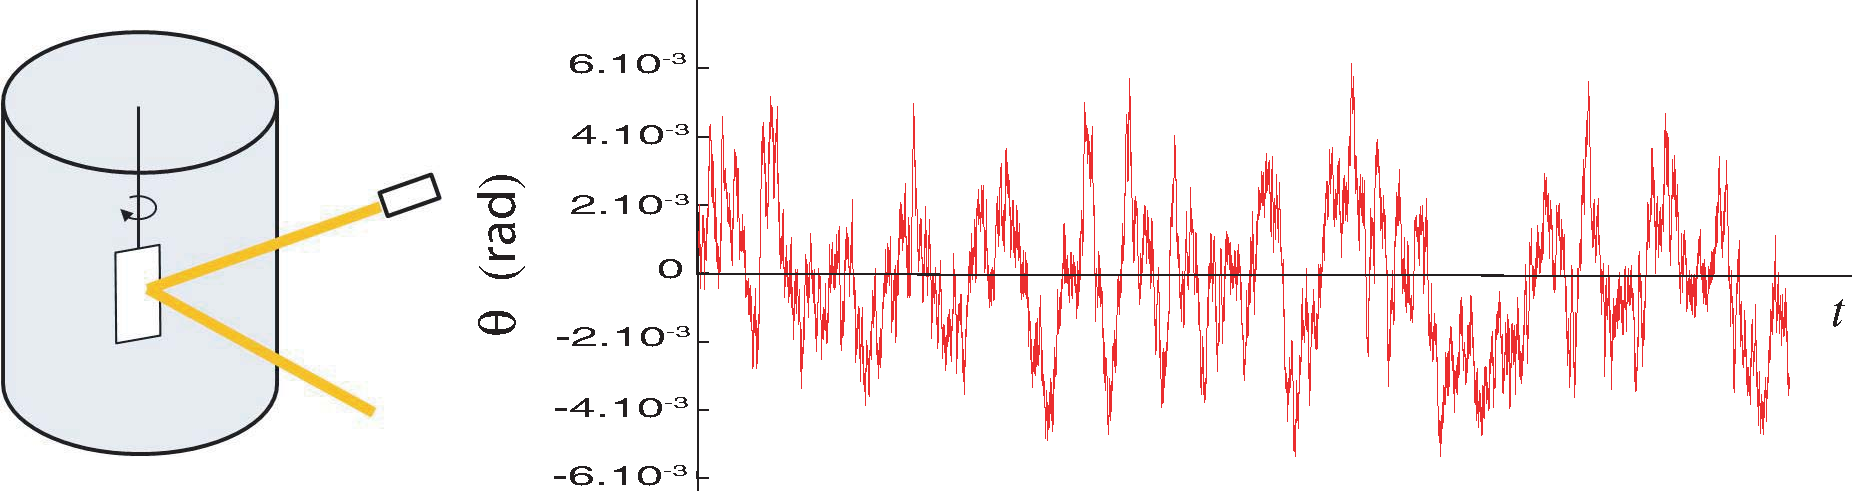
\includegraphics{kappler}}
\caption{\it \`A gauche : schéma de l'expérience de Kappler. \`A
  droite : exemple de courbe $\theta(t)$ obtenue en enregistrant la
  déviation du faisceau lumineux au cours du temps.\label{FigKappler}}
\end{center}
\end{figure}


\question
Pour quelle raison le miroir effectue-t-il de petites oscillations autour de sa position d'équilibre ? 

\question
\'Ecrire la distribution de probabilité $P(\theta)$ de l'angle de rotation.  Calculer $\langle {\theta} \rangle$ et Var$(\theta)$.

\question
\`A partir de la courbe $\theta(t)$ reportée sur la figure \ref{FigKappler}, estimer l'écart type de $\theta$. La raideur du fil est $K\simeq 10^{-15}$\,J.rad$^{-2}$ et la température $T\simeq 300$ K. En déduire une valeur estimée de la constante de Boltzmann. 
  


% ______________________________________________________________________________
\section{\hard~Le modèle d'Einstein}

Einstein fut le premier à proposer en 1907 un modèle capable de rendre compte du comportement des capacités calorifiques des solides à basse température : leur diminution sensible, en contradiction avec la loi classique de Dulong et Petit.

Voici le modèle : on admet que chaque atome du solide vibre indépendamment des autres atomes à la même pulsation $\omega $ dans chacune des trois directions possibles. Le solide, formé de $N$ atomes est donc équivalent à un ensemble de
$3N$ oscillateurs à une dimension indépendants de pulsation propre $\omega$. On sait que les états propres de l'Hamiltonien de chacun de ces oscillateurs ont des niveaux discrets non dégénérés d'énergie $\epsilon_n$ caractérisée par un nombre quantique $n$ ($n=0,1,2,3\ldots$) telle que
$$
  \epsilon_n=(n+\frac{1}{2}) \hbar \omega.
$$

Dans tout ce qui suit, on suppose que le solide est en équilibre thermique avec un thermostat à la température $T$. On pourra introduire la grandeur $\theta=\hbar \omega/k_B$ que l'on interprétera.

\question
Rappeler le lien entre la fonction de partition d'un système en équilibre thermique avec son énergie libre, son énergie interne (i.e. son énergie moyenne), puis sa capacité calorifique à volume constant.

\question Calculer la fonction de partition $z$ d'un oscillateur harmonique quantique à une dimension (pour calculer la somme on remarquera qu'il s'agit d'une simple série géométrique).

\question Calculer l'énergie moyenne $\overline \epsilon (T)$ de cet oscillateur. Tracer qualitativement $\overline \epsilon (T)$ en fonction de $T$. Quelle est l'énergie interne $\overline E$ du solide dans le cas du modèle d'Einstein ?

\question Dans la limite où $T \ll \theta$, sans aucun calcul, que peut-on dire de la valeur de $\overline E$ ? Vérifier-le sur la formule précédente.

\question Dans la limite où $T \gg \theta$, que vaut $\overline E$ ? Comment dépend-elle de $T$ ? de $\omega $ ? 

\question Montrer que dans le modèle d'Einstein, la capacité calorifique molaire à volume constant $C_V$ du solide est égale à
$$
 C_V=3R \frac{x^2 \exp ( x)}{[\exp (x)-1]^2}
$$
ou $R$ est la constante des gaz parfaits et $\displaystyle{x=\frac{\theta}{T}}$.

\question
Tracer sommairement $C_V(T)$en fonction de $T$. \'Etudier en particulier les limites $C_V(T \to + \infty)$, puis $C_V(T \to 0)$. Donner une expression approchée de $C_V(T)$ quand $T \ll \theta$.

\question
On donne à 298 K pour le cuivre $\theta=230$K et $C_V=23,8$ J.K$^{-1}$.mol$^{-1}$ tandis que pour le diamant $\theta=830$ K et $C_V=6.1$ J.K$^{-1}$.mol$^{-1}$. Commenter.



\end{document}
